\setlength{\columnsep}{3pt}
\begin{flushleft}
	\bigskip
	\textbf{stat}: Check file permissions and more details like access time, modify time \& change time.
	\bigskip
	\begin{tcolorbox}[breakable,notitle,boxrule=0pt,colback=pink,colframe=pink]
		\color{black}
		\fontdimen2\font=1em
		Syntax: stat  file\_or\_directory\_name
		\fontdimen2\font=4pt
	\end{tcolorbox}
	
	Eg:
	\begin{figure}[h!]
		\centering
		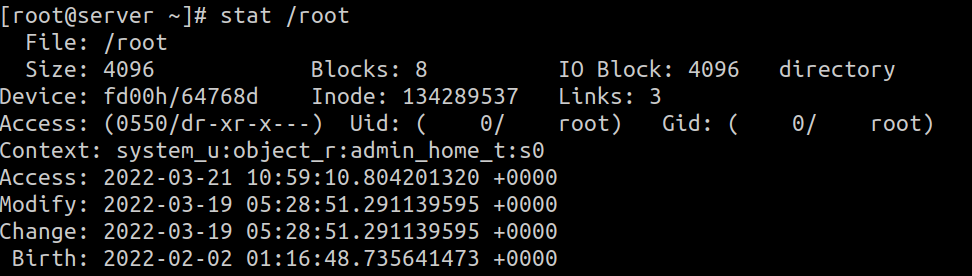
\includegraphics[scale=0.4]{content/chapter5/images/stat.png}
		\caption{Sample output}
		\label{fig:sample2}
	\end{figure}
	
	\textbf{ls -ld}: Check file permission and details like file owner, group owner \& timestamp.
	\bigskip
	\begin{tcolorbox}[breakable,notitle,boxrule=0pt,colback=pink,colframe=pink]
		\color{black}
		\fontdimen2\font=1em
		Syntax: ls -ld  file\_or\_directory\_name
		\fontdimen2\font=4pt
	\end{tcolorbox}
	
	Eg:
	\begin{figure}[h!]
		\centering
		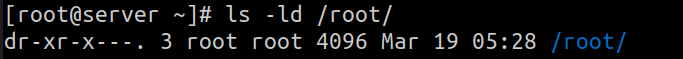
\includegraphics[scale=0.6]{content/chapter5/images/ls.png}
		\caption{Sample output}
		\label{fig:sample3}
	\end{figure}
	
	
	\newpage
	
	
	\textbf{chmod}: Change the permission of a file or directory using either the octal representation 
	or symbolic representation.
	\bigskip
	\begin{tcolorbox}[breakable,notitle,boxrule=0pt,colback=pink,colframe=pink]
		\color{black}
		\fontdimen2\font=1em
		Syntax: chmod  permission  file\_or\_directory\_name
		\fontdimen2\font=4pt
	\end{tcolorbox}
	
	The permission in chmod command can be supplied using:
	\begin{itemize}
		\item Octal representation
		\item Symbolic representation
	\end{itemize}

	Let's see each of these in detail.

\newpage
\paragraph{Octal representation}

\begin{figure}[h!]
	\centering
	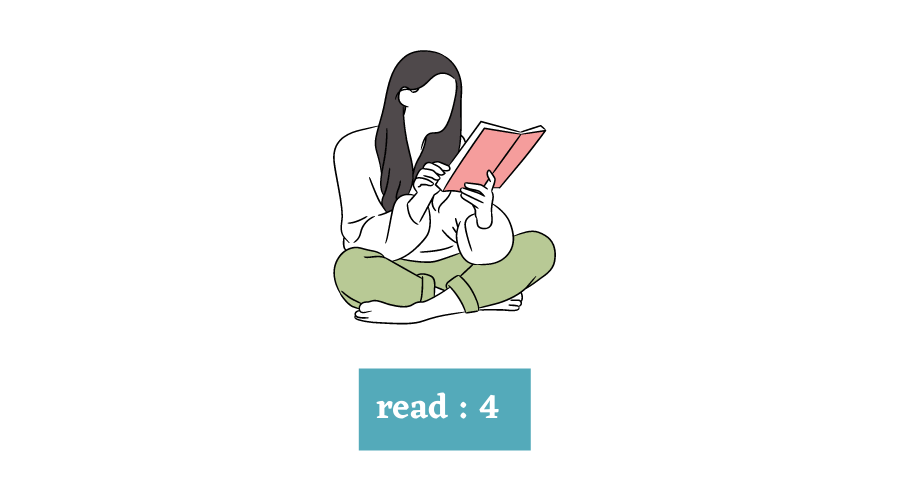
\includegraphics[scale=0.4]{content/chapter5/images/67.png}
	\caption{Octal representation of read}
	\label{fig:read}
\end{figure}

\begin{figure}[h!]
	\centering
	
\includegraphics[scale=0.4]{content/chapter5/images/68.png}
	\caption{Octal representation of write}
	\label{fig:write}
\end{figure}

\begin{figure}[h!]
	\centering
	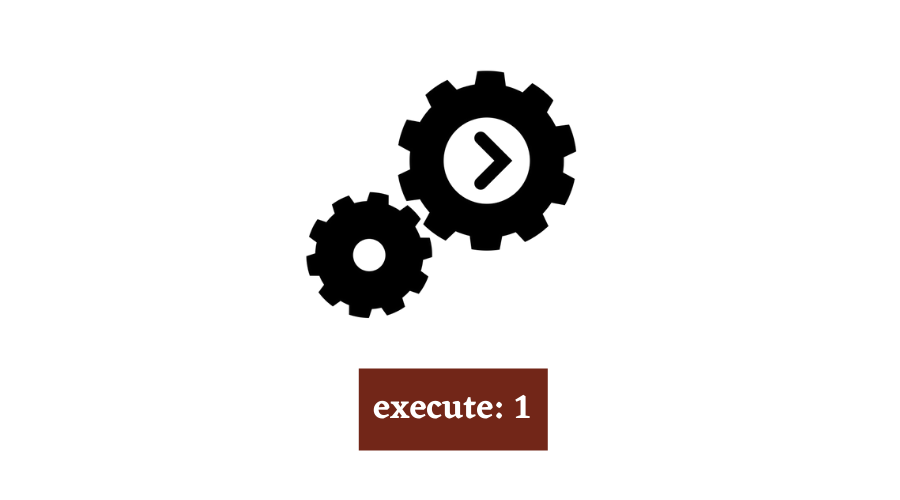
\includegraphics[scale=0.4]{content/chapter5/images/69.png}
	\caption{Octal representation of execute}
	\label{fig:execute}
\end{figure}

\newpage

Let's review the different combinations. Observe the letter representation, the octal representation, and the meaning in the shown image:

\begin{figure}[h!]
	\centering
	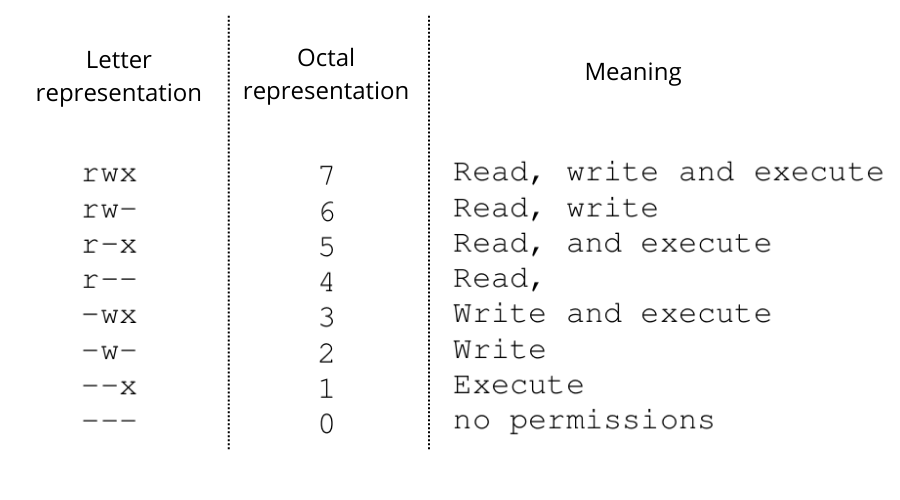
\includegraphics[scale=0.4]{content/chapter5/images/perm4.png}
	\caption{Permission octal representation}
	\label{fig:combination_permission1}
\end{figure}

Octal permission combination for user, group \& other can be as follows:

\begin{figure}[h!]
	\centering
	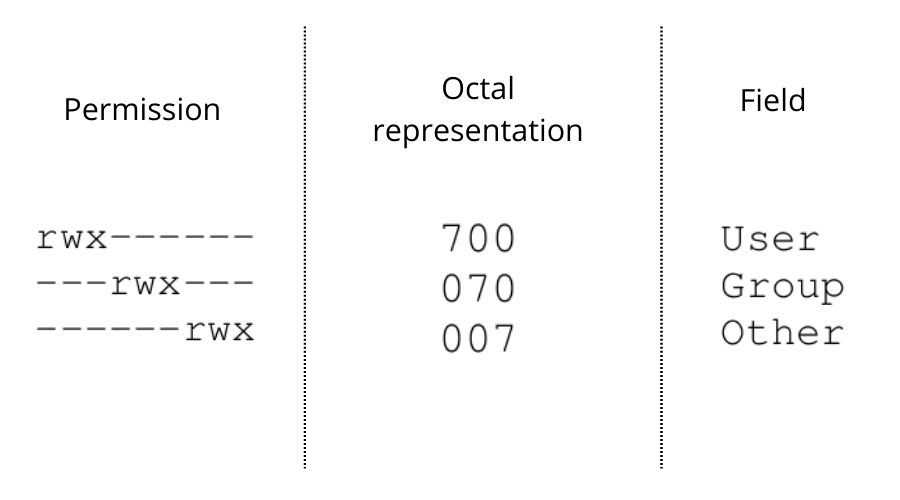
\includegraphics[scale=0.4]{content/chapter5/images/perm5.png}
	\caption{Permission combination}
	\label{fig:combination_permission2}
\end{figure}


\newpage
Egs:
	\begin{itemize}
		\item 	Give read, write ( 4+2 = 6 ) to user and read ( 4 ) to group and others.
		\begin{tcolorbox}[breakable,notitle,boxrule=-0pt,colback=black,colframe=black]
			\color{green}
			\fontdimen2\font=1em
			\# chmod 644 filename
			\fontdimen2\font=4pt
		\end{tcolorbox}
		\bigskip
		
		\item Give read, execute ( 4 + 1 = 5 ) to user and read (4 ) to group, and nothing ( 0 ) to others.
		\bigskip
		\begin{tcolorbox}[breakable,notitle,boxrule=-0pt,colback=black,colframe=black]
			\color{green}
			\fontdimen2\font=1em
			\# chmod 540 filename
			\fontdimen2\font=4pt
		\end{tcolorbox}

	\bigskip
	\item Give read, write ( 4 + 2 = 6 ) to user and nothing ( 0 ) to group, and read ( 4 ) to others.
	\bigskip
	\begin{tcolorbox}[breakable,notitle,boxrule=-0pt,colback=black,colframe=black]
		\color{green}
		\fontdimen2\font=1em
		\# chmod 604 filename
		\fontdimen2\font=4pt
	\end{tcolorbox}
	\end{itemize}

	\newpage
	\paragraph{Symbolic representation}
	\bigskip
	Below image shows all the symbols used in permission:
	\begin{figure}[h!]
		\centering
		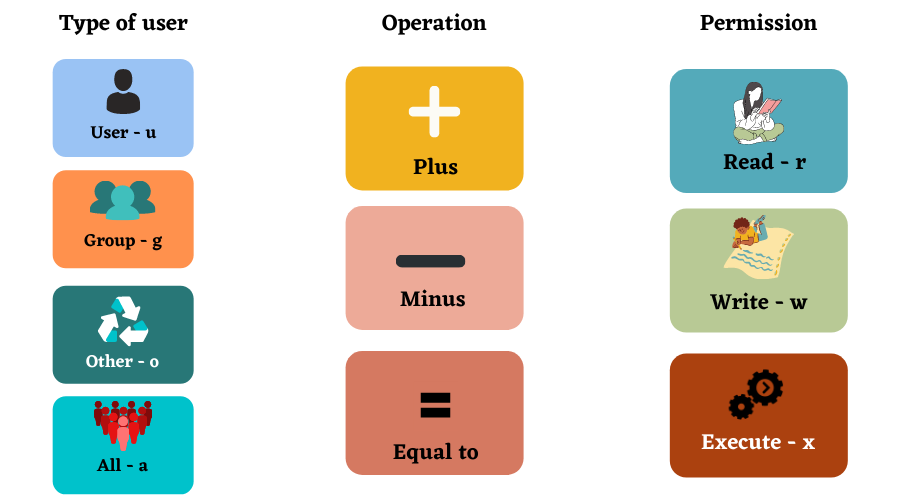
\includegraphics[scale=0.6]{content/chapter5/images/perm8.png}
		\bigskip
		\caption{Symbolic representation to assign permissions}
		\label{fig:assign_permission}
	\end{figure}
	
	Symbols here indicates:
	\begin{itemize}
		\item \textbf{u} : User
		\item \textbf{g} : Group
		\item \textbf{o} : Other
		\item \textbf{a} : All
		\item \textbf{+} : Add permission
		\item \textbf{-} : Remove permission
		\item \textbf{=} : Assign permission
		\item \textbf{r} : Read
		\item \textbf{w} : Write
		\item \textbf{x} : Execute
	\end{itemize}


	
	

	\newpage
	Let's see some of the examples to understand how we can use the symbolic representation.
	\begin{itemize}
	\item Assign user, group and other with read and write permission.
	\begin{tcolorbox}[breakable,notitle,boxrule=-0pt,colback=black,colframe=black]
		\color{green}
		\fontdimen2\font=1em
		\# chmod =rw myfile
		\newline
		or
		\newline
		\# chmod u=rw myfile
		\newline
		\# chmod g=rw myfile
		\newline
		\# chmod o=rw myfile
		\fontdimen2\font=4pt
	\end{tcolorbox}
	\bigskip
		
	\item Remove read and write permission for other.
	\begin{tcolorbox}[breakable,notitle,boxrule=-0pt,colback=black,colframe=black]
		\color{green}
		\fontdimen2\font=1em
		\# chmod o-rw myfile
		\fontdimen2\font=4pt
	\end{tcolorbox}
	\bigskip

	\item Add read and remove write permission from group.
	\begin{tcolorbox}[breakable,notitle,boxrule=-0pt,colback=black,colframe=black]
		\color{green}
		\fontdimen2\font=1em
		\# chmod g+r-w myfile
		\fontdimen2\font=4pt
	\end{tcolorbox}
	\bigskip

	\item Assign group with read permission, remove write permission from group. Assign other with read,write \& execute permission.
	\begin{tcolorbox}[breakable,notitle,boxrule=-0pt,colback=black,colframe=black]
		\color{green}
		\fontdimen2\font=1em
		\# chmod g+r-w,o=rwx myfile
		\fontdimen2\font=4pt
	\end{tcolorbox}
	\bigskip

	\item Assign read, write permission to user, group \& other.
	\begin{tcolorbox}[breakable,notitle,boxrule=-0pt,colback=black,colframe=black]
		\color{green}
		\fontdimen2\font=1em
		\# chmod a=rw myfile
		\newline
		or
		\newline
		\# chmod =rw myfile
		\fontdimen2\font=4pt
	\end{tcolorbox}

\end{itemize}

\newpage

\paragraph{Command to change user and group ownership}
\bigskip
\textbf{chown}: Changes the user and group ownership of for given file or directory.

\begin{tcolorbox}[breakable,notitle,boxrule=0pt,colback=pink,colframe=pink]
	\color{black}
	\fontdimen2\font=1em
	Syntax: chown username file\_or\_directory
	\newline
	Syntax: chown username:groupname file\_or\_directory
	\fontdimen2\font=4pt
\end{tcolorbox}

Egs:
\begin{itemize}
	\item Change file ownership to natasha user.
	\begin{tcolorbox}[breakable,notitle,boxrule=-0pt,colback=black,colframe=black]
		\color{green}
		\fontdimen2\font=1em
		\# chown natasha demo.txt
		\fontdimen2\font=4pt
	\end{tcolorbox}	
	\bigskip

	\item Change file ownership to natasha user and group ownership to devops.
	\begin{tcolorbox}[breakable,notitle,boxrule=-0pt,colback=black,colframe=black]
		\color{green}
		\fontdimen2\font=1em
		\# chown natasha:devops demo.txt
		\fontdimen2\font=4pt
	\end{tcolorbox}
	\bigskip

\end{itemize}

Options with \textbf{chown} command:	
\newline
\textbf{-R}: Recursively change ownership of directories and their contents.
\begin{tcolorbox}[breakable,notitle,boxrule=0pt,colback=pink,colframe=pink]
	\color{black}
	\fontdimen2\font=1em
	Syntax: chown -R username directory
	\newline
	Syntax: chown -R username:groupname directory
	\fontdimen2\font=4pt
\end{tcolorbox}
\newline
Eg: Change the owner of a directory and it's subfiles to "shammy".
\begin{tcolorbox}[breakable,notitle,boxrule=-0pt,colback=black,colframe=black]
	\color{green}
	\fontdimen2\font=1em
	\# chown -R shammy /foo
	\fontdimen2\font=4pt
\end{tcolorbox}


\newpage

\paragraph{Command to change group ownership}
\bigskip
\textbf{chgrp}: Changes the group ownership for given file or directory.

\begin{tcolorbox}[breakable,notitle,boxrule=0pt,colback=pink,colframe=pink]
	\color{black}
	\fontdimen2\font=1em
	Syntax: chgrp groupname file\_or\_directory
	\fontdimen2\font=4pt
\end{tcolorbox}

Eg: Change file \textbf{"demo.text's"} group ownership to \textbf{"devops"} group.
\begin{tcolorbox}[breakable,notitle,boxrule=-0pt,colback=black,colframe=black]
		\color{green}
		\fontdimen2\font=1em
		\# chgrp devops demo.txt
		\fontdimen2\font=4pt
\end{tcolorbox}
	
Options with \textbf{chgrp} command:	
\newline
\textbf{-R}: Recursively change ownership of directories and their contents.
\begin{tcolorbox}[breakable,notitle,boxrule=0pt,colback=pink,colframe=pink]
	\color{black}
	\fontdimen2\font=1em
	Syntax: chgrp -R groupname directory
	\fontdimen2\font=4pt
\end{tcolorbox}
Eg: Change the groupname of \textbf{"/foo"} directory and it's subfiles/subfolders to "devops" group.
\begin{tcolorbox}[breakable,notitle,boxrule=-0pt,colback=black,colframe=black]
	\color{green}
	\fontdimen2\font=1em
	\# chgrp -R devops /foo
	\fontdimen2\font=4pt
\end{tcolorbox}


	
\end{flushleft}

\newpage

